\section{Unbiased $f_i$ Estimation}
\label{sec:unbiased-estimate}

Based on our observations in the previous section we will alter Kmerlight 
to produce unbiased estimates of $f_i$.

To achieve an unbiased estimate of $f_i$ we fix the value of $w^*$. 
With this alteration, Kmerlight will no longer choose the level
that maximzes the number of collision-free counters, but the level that maximizes
the expected number number of collision-free counters.

Since the expected number of collision-free counters is the same for all abundancies
$i=1,2,\dots m$, the level $w^*$ from which the estimate $\hat f_i$ will be calculated
will be the same for all abundancies.

The value $w^*$ can be calculated using only the number of all distinct
$k$-mers ($F_0$) and the number of counters at each level ($r$ ).

Firstly, Kmerlight with fixed $w^*$ processes all the $k$-mers in the same
way as the original Kmerlght did. Then $F_0$ is estimated and the
value is $w^*$ calculated to maximize the expected number of
collision-free counters as it was described in section \ref{sec:analytical-w}.
Finally, values of $f_i$ are estimated from the observed counts of 
collision-free counters at level $w^*$.

In figures \ref{img:mean-new-algorithm} and \ref{img:std-new-algorithm} we present the comparison
of the original Kmerlight and Kmerlight with fixed $w^*$. Our new algorithm removes bias
and maintains the same accuracy (variance) of the estimates.


\begin{figure}
\centerline{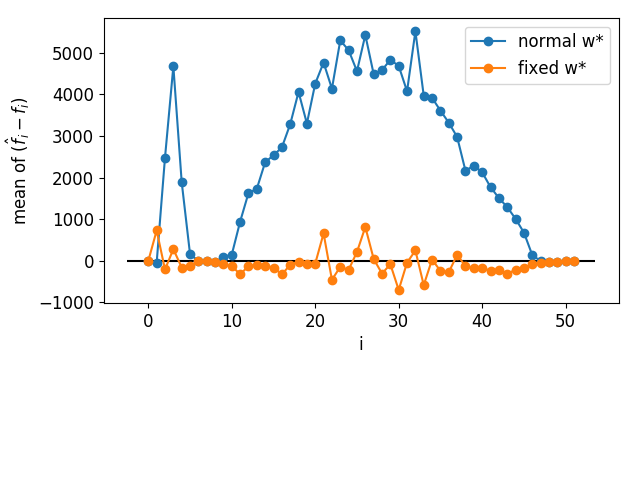
\includegraphics[width=0.8\textwidth, trim={0cm, 3cm, 0cm, 0cm}, clip]{images/means_comparison.png}}
\caption[Mean error of normal Kmerlight and Kmerlight with fixed $w^*$]{Mean errors of estimates
($\hat f_i - f_i$) from 50 trials. While the original Kmerlight overestimates 
$f_i$ significantly in an average run, Kmerlight with fixed $w^*$ achieves $E(\hat f_i) \approx f_i$.}
\label{img:mean-new-algorithm}
\end{figure}

\begin{figure}
\centerline{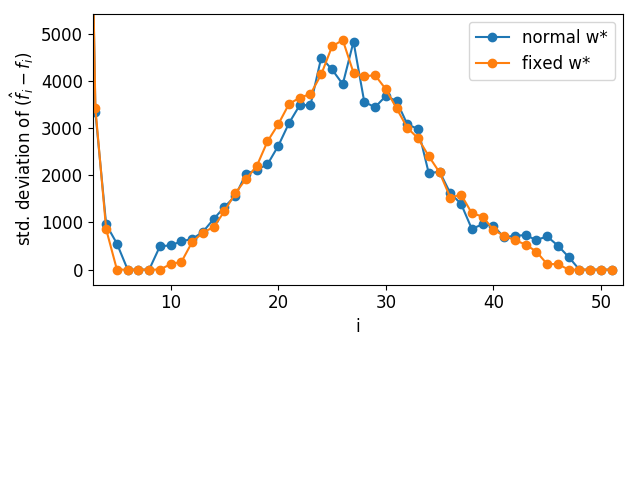
\includegraphics[width=0.8\textwidth, trim={0cm, 3.5cm, 0cm, 0cm}, clip]{images/std_deviations_comparison.png}}
\caption[Variance of normal Kmerlight and Kmerlight with fixed $w^*$]{Standard deviation of estimates
($\hat f_i - f_i$) from 50 trials. The alteration in Kmerlight does not change the variance of estimates}
\label{img:std-new-algorithm}
\end{figure}

